\let\negmedspace\undefined
\let\negthickspace\undefined
\documentclass[journal]{IEEEtran}
\usepackage[a5paper, margin=10mm, onecolumn]{geometry}
%\usepackage{lmodern} % Ensure lmodern is loaded for pdflatex
\usepackage{tfrupee} % Include tfrupee package
\setlength{\headheight}{1cm} % Set the height of the header box
\setlength{\headsep}{0mm}     % Set the distance between the header box and the top of the text
\usepackage{gvv-book}
\usepackage{gvv}
\usepackage{cite}
\usepackage{amsmath,amssymb,amsfonts,amsthm}
\usepackage{algorithmic}
\usepackage{graphicx}
\usepackage{textcomp}
\usepackage{xcolor}
\usepackage{txfonts}
\usepackage{listings}
\usepackage{enumitem}
\usepackage{mathtools}
\usepackage{gensymb}
\usepackage{comment}
\usepackage[breaklinks=true]{hyperref}
\usepackage{tkz-euclide} 
\usepackage{listings}
% \usepackage{gvv}                                        
\def\inputGnumericTable{}                                 
\usepackage[latin1]{inputenc}                                
\usepackage{color}                                            
\usepackage{array}                                            
\usepackage{longtable}                                       
\usepackage{calc}                                             
\usepackage{multirow}                                         
\usepackage{hhline}                                           
\usepackage{ifthen}                                           
\usepackage{lscape}
\begin{document}

\bibliographystyle{IEEEtran}
\vspace{3cm}
\parindent 0px

\title{9.2.3}
\author{EE24BTECH11050 - Pothuri Rahul}
% \maketitle
% \newpage
% \bigskip
{\let\newpage\relax\maketitle}

\renewcommand{\thefigure}{\theenumi}
\renewcommand{\thetable}{\theenumi}
\setlength{\intextsep}{10pt} % Space between text and floats


\numberwithin{equation}{enumi}
\numberwithin{figure}{enumi}
\renewcommand{\thetable}{\theenumi}

\textbf{Question:} \\
What is the solution for the differential equation $y'+\sin{x}=0$
\solution \\
\textbf{Theoretical solution :} \\
by rearranging the given differential equation \\
\begin{align}
\frac{dy}{dx} = - \sin{x} \label{1}
\end{align}
On integrating both sides w.r.to x,
\begin{align}
\int \frac{dy}{dx} dx = \int \brak{- \sin{x}} dx \\
y = \cos{x}+C
\end{align}
\textbf{Solution using Trapezoidal rule :} \\
Consider the equation \eqref{1},
\begin{align}
\frac{dy}{dx} = - \sin{x} \\
dy = -\sin{x}dx
\end{align}
To apply the Trapezoidal rule, we need to convert it into definite integration. For that let us take two points on x-axis $x_n$ and $x_{n+1}$,which are at a small separation h and $y_n , y_{n+1}$ be the values of respectively. \\
\begin{align}
\int\limits_{y_n} ^{y_{n+1}} dy = - \int\limits_{x_n} ^{x_{n+1}} \sin{x} dx
\end{align}
By Trapezoidal rule,We can approximate it as,
\begin{align}
y_{n+1}-y_n = - \frac{1}{2} \times h \brak{ \sin{x_n}+\sin{x_{n+1}}} \\
y_{n+1} = y_n- \frac{1}{2} \times h \brak{ \sin{x_n}+\sin{x_{n+1}}}
\end{align}
Where,
\begin{align}
h = x_{n+1} - x_n
\end{align}
By taking initial conditions as $x_0 = 0,y_0 = 1$ and plotting the points resulted in this algorithm will give the approximate graph for the given differential equation \eqref{1} \\

\textbf{Solution using Bilinear :} \\
Apply laplace tranform for \eqref{1} \\
\begin{align}
\frac{dy}{dx} = - \sin{x} \\
y' = - \sin{x} \\
\mathcal{L} \brak{y'} = \mathcal{L} \brak{ - \sin{x} } \label{2}
\end{align}
Let 
\begin{align}
\mathcal{L} \brak{y} = Y(S)\\
\end{align}
Then 
\begin{align}
\mathcal{L} \brak{y'} = sY(s) - y_0
\end{align}
From \eqref{2}
\begin{align}
sY(s) - y_0 = -\frac{1}{s^2+1} \\
Y(s) = \frac{1}{s} \brak{y_0 - \frac{1}{s^2+1}}  \label{3}
\end{align}
By taking initial conditions, y = 1 in \eqref{3}
\begin{align}
Y(s) = \frac{1}{s} - \frac{1}{s\brak{s^2+1}} \\
Y(s) = \frac{s}{s^2+1} \label{3}
\end{align}
let us convert the equation \eqref{3} to Z-domain from s-domain by using the bilinear tranform technique. \\
For that we have to substitute 
\begin{align}
s = \frac{2}{h} \frac{1-z^{-1}}{1+z^{-1}}
\end{align}
Then,
\begin{align}
Y(z) = \frac{\frac{2}{h} \frac{1-z^{-1}}{1+z^{-1}}}{\brak{\frac{2}{h} \frac{1-z^{-1}}{1+z^{-1}}}^2+1}
\end{align}
On simplifying,We get 
\begin{align}
Y(z) = \frac{2h\brak{z^2-1}}{z^2\brak{4+h^2}+2z\brak{h^2-4}+\brak{4+h^2}} \label{4}
\end{align} \\ \\ 
We need to find the inverse of this equation to get a difference equation,For that let us use the following properties of the z-transform 
\begin{align}
    \mathcal{Z}\brak{y\sbrak{n + 2}} &= z^2 Y\brak{z} - y\sbrak{1}z - y\sbrak{0}\\
    \mathcal{Z}\brak{y\sbrak{n + 1}} &= z Y\brak{z} - z y_\sbrak{0}\\
    \mathcal{Z}\brak{\delta\sbrak{n}} &= 1 \text{, } z \neq 0\\
\end{align}
By the time shift property 
\begin{align}
    \mathcal{Z}\brak{\delta\sbrak{n + 2}} &= z^2 \text{, } z \neq 0\\
    \mathcal{Z}\brak{\delta\sbrak{n + 1}} &= z \text{, } z \neq 0
\end{align}
By rearranging the terms in equation \eqref{4} \\
\begin{align}
z^2\brak{4+h^2} Y(z) +2z\brak{h^2-4} Y(z) +\brak{4+h^2} Y(z) = 2h\brak{z^2-1} 
\end{align}
\begin{align}
z^2 Y(z) + 2z \frac{h^2-4}{h^2+4}Y(z) +Y(z) = \frac{2h\brak{z^2-1}}{4+h^2} \label{5}
\end{align}
Let us adjust the following equation \eqref{5} to get into standard forms,
\begin{align}
z^2 Y(z) -y_1z-y_0 + 2z \frac{h^2-4}{h^2+4}Y(z) - 2z \frac{h^2-4}{h^2+4}y_0  +Y(z) = \frac{2h\brak{z^2-1}}{4+h^2} -y_1z-y_0 - 2z \frac{h^2-4}{h^2+4}y_0 
\end{align}
\begin{align}
\brak{z^2 Y(z) -y_1z-y_0} + 2\frac{h^2-4}{h^2+4} \brak{zY(z) - zy_0} +Y(z) = z^2 \brak{\frac{2h}
{h^2+4}} - z \brak{y_1 + 2y_0 \frac{h^2-4}{h^+4}} - \brak{\frac{2h}{h^2+4} + y_0} \label{6}
\end{align}
where $z \neq 0$ \\
Region of convergence \brak{ROC} is given by $z \neq 0$ \\
by using properties,Inversing of the above equation \eqref{6} will result as the following ,
\begin{align}
y_{n+2} + \frac{2\brak{h^2-4}}{h^2+4} y_{n+1} + y_n = \frac{2h}{h^2+4} \delta \sbrak{n+2} - \brak{y_1 + 2y_0 \frac{h^2-4}{h^+4}} \delta \sbrak{n+1} - \brak{\frac{2h}{h^2+4} + y_0} \delta \sbrak{n} \label{7}
\end{align}
Where $\delta$ is defined as following,
\begin{align}
    \delta\sbrak{n - n_0} =
    \begin{cases}
        1 & \quad n = n_0\\
        0 & \quad n \neq n_0
    \end{cases}
\end{align}
As $n > 0$ , 
\begin{align}
\delta \sbrak{n+1} = 0 \\
\delta \sbrak{n+2} = 0
\end{align}
Then \eqref{7} becomes as 
\begin{align}
y_{n+2} + \frac{2\brak{h^2-4}}{h^2+4} y_{n+1} + y_n = - \brak{\frac{2h}{h^2+4} + y_0} \delta \sbrak{n}
\end{align} 
To get $y_1$, Let us use the defination of the differentiation,
\begin{align}
y' \approx \frac{y_{n+1} - y_n}{h}
\end{align}
For n = 0 \\
\begin{align}
y' = \frac{y_1 - y_0}{h} \\
y_1 = y_0 + hy'
\end{align}
We need to plot all these resulting points, to get the graph of thr solution of differential equation \eqref{1} 


\begin{figure}[htbp] % Positioning options: here, top, bottom, page
    \centering
    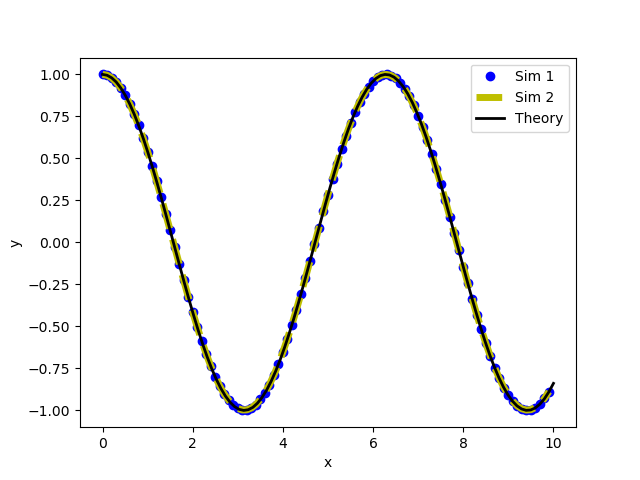
\includegraphics[width=\textwidth]{figs/plot.png} % Replace "filename" with your image file
    \caption{Plot}
\end{figure}






\end{document}
